\section{Menu and Shortcuts}
The layout of the standard menu structure has been fixed for a great many years, and in creating this application we have tried to stick to these conventions.  We have implemented a "File" menu containing "Open", "Save", and "Exit" commands; we created an "Edit"  menu with add and delete annotation commands; and we have a "View" menu where the user can control which docks they wish to see, and at which zoom level the image viewer should be set.  There isn’t a great deal that can be said for this particular layout, nearly every application has had these menu items in this precise order for at least the past fifteen years, except to mention that in terms of human computer interactions, and where a user expects commands to be located, a GUI designer should ignore this convention at their peril.

\begin{figure}[h]
\centering
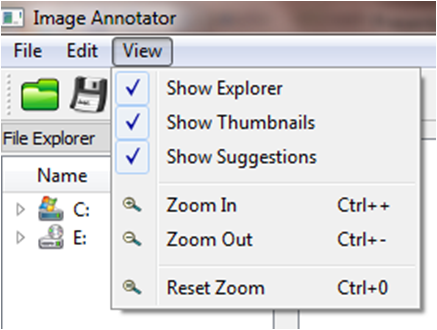
\includegraphics[width=6cm]{menu.png}
\caption{A screen-shot of our main menu showing File, Edit and View sub-menus}
\label{fig:fullView}
\end{figure}

We have tried to stick to convention again when choosing the shortcut keys for the main menu items, particularly when it came to the file system commands.  The items file, open, save, and exit usually the have same keyboard bindings in all applications and so we have not altered this since we do not wish to confuse the user.  As previously mentioned, the bindings for the zoom feature have been taken from those present in most Internet browsers.  In terms of software, these applications are amongst the most used on a computer today: thus following their standards seemed wise.  Unfortunately when it came to the annotation commands there were no such well-known templates to follow, and so it was down to common sense to provide the answer.  Add annotation begins with the letter a and so that was chosen to represent that action.  Following the same logic the letter d might have been chosen for the delete action, except that the QWERTY keyboard layout already has two keys dedicated to this task - delete and backspace.  In the end, backspace was chosen since it is more familiar to unsophisticated users and hence they are more likely to associate it with a delete action.

We also included a status bar at the bottom of the application.  This displays context-sensitive text depending upon where the mouse is hovering.  This is common in many applications and we hope that this will aid users in the use of this package.
